\documentclass[../main_config.tex]{subfiles}
\begin{document}



\chapter{Aufnahme der Messergebnisse}
Bevor die ersten Messungen am System gemacht werden können, muss diese ausreichend auf ihre Funktionsfähigkeit getestet werden. Aufgrund der langen Lieferzeit der bestellten Bauteile gab es im Vorfeld ausreichend Zeit ein kleines Testprotokoll zu erarbeiten.\par


\section{Funktionstest der Leiterplatte}
Nach Fertigstellung des \gls{pcb} wird zunächst der aufkommende Versorgungsstrom auf einen definierten Wert begrenzt. Anschließend wird kontrolliert, ob der Buck-Converter die \SI{3.3}{\volt} zuverlässig ausgibt. Sobald das funktioniert, kann die Ansteuerung der Digitalpotentiometer durch die \gls{mcu} programmiert werden. Mithilfe der zuvor geplanten Jumper kann der daraus resultierende Widerstandswert unabhängig von der Restschaltung gemessen und der Code dadurch validiert werden. \par
\medskip

Im nächsten Schritt könnten die fehlenden \glspl{ic} gesteckt werden um das Gesamtsystem zu vermessen. Da die Reaktion des Systems jedoch noch nicht genau bekannt ist, werden die Multiplizierer erst einmal überbrückt, um nur den bereits bekannten Biquad aufzunehmen. Der Phase-Detektor kann dabei vorerst vernachlässigt werden. Stimmen diese Ergebnisse mit den früheren Resultaten überein, kann anschließend das vollständige System vermessen werden. \par
\medskip

Auffällig ist, dass die \gls{mcu} bei anlegen der Versorgungsspannung nicht immer zuverlässig bootet. Ein möglicher Grund hierfür könnte eine nicht ausreichend stabilisierte Versorgungsspannung sein. Lösungsansätze sind zum Beispiel das Einsetzen eines Stützkondensators am $V_{sys}$-Eingang oder das Hinzufügen eines Schalters am \SI{3.3}{\volt}-Jumper. Sobald die \SI{\pm15}{\volt} erst einmal anliegen kann der Schalter gesetzt werden wonach die \gls{mcu} zuverlässig startet. Um auf Anhieb zu erkennen, dass der Pico ordnungsgemäß hochfährt, wird das Skript erweitert, sodass die Onboard-LED als Statusindikator fungiert.\par
\medskip




\subsection{Kompensation der Widerstandsabweichungen in den Digitalpotentiometern}

Bei der ersten Messung des herkömmlichen Biquads ohne Self-Tune-System zeigt sich eine deutliche Abweichung der Mittenfrequenz von der in der \gls{ui} eingestellten Frequenz. Dabei gibt es sowohl eine Diskrepanz zwischen dem theoretischen Sollwert \text{soll\_R} und dem durch den Wiper eingestellten Istwert \text{ist\_R}, als auch eine Abweichung zwischen dem Istwert und dem real abfallenden Widerstandswert. \par
\medskip

Die Abweichung zwischen dem Ist- und Sollwert ist recht einfach zu erklären. Das verwendete Potentiometer wird über ein \num{8}-Bit Steuerregister angesteuert, dass nur $2 ^8= 256$ diskrete Zustände annehmen kann. Diese Zustände sind gleichmäßig über den gesamten Widerstandsbereich verteilt, was zu einer konstanten Schrittweite führt. Die Gleichung\par
\medskip

\begin{equation}
    R_{step} = \frac{R_{max}-R_{min}}{2^{n}-1} = \frac{\SI{9980}{\ohm}-\SI{150}{\ohm}}{255} = \SI{38.5}{\ohm}
\end{equation}

beschreibt die Zusammensetzung der Schrittweite, wobei
\begin{itemize}
    \item $R_{max}$ den größt möglichen Widerstand darstellt,
    \item $R_{min}$ den kleinst möglichen Widerstand angibt.
\end{itemize}

Der Abstand zwischen zwei einstellbaren Widerstandswerten beträgt also $R_{step}=\SI{38}{\ohm}$. Bei der Umrechung eines gewünschten Widerstandswerts in einen \num{8}-Bit Wert, muss dieser auf den Bereich von \num{0} bis \num{255} normiert werden. Da der normierte Wert seltenst einer Ganzzahl entspricht, wird dieser im Skript anschließend noch gerundet. So addieren sich zur Abweichung durch die Schrittweite zusätzlich Rundungsfehler, die die Differenz zwischen Ist- und Sollwert erhöhen. \par
\medskip

%Dies beeinträchtigt stark die Differenz zwischen dem Idealwert und dem aus den Funktionen errechneten Wert. Wenn nun also ein bestimmter widerstandswert, zum Beispiel \SI{1}{\kilo\ohm}, eingestellt werden, muss dieser wert erst auf die \num{255} Steps normiert werden, die über den \gls{spi}-Bus übertragen werden können. Dabei kann es passieren, das der Wert nicht als Ganzzahl ausgegeben werden kann. Die zweite Fehlerquelle basiert also auf dem Ruden des Bitwerts für die Einstellung des Widerstandswerts. Diese addiert sich zu der ersten fehlerqelle.

Die Diskrepanz zwischen dem eingestellten Istwert und dem tatsächlich gemessenen Realwert ist nicht so einfach zu ermitteln. Darum wird im Folgenden kurz untersucht, ob die anfallenden Abweichungen durch Anpassungen im Skript kompensiert werden können. Dafür werden die Widerstände für den Ist- und Sollwert über das \gls{ui} ausgegeben. Gleichzeitig wird der Widerstand des Potentiometers \num{1} über ein Multimeter gemessen. Auf eine Messung der anderen Potentiometer wird hierbei verzichtet, da ihre Werte immer innerhalb von \SI{10}{\ohm} übereinstimmten. Die gemessenen Werte sind in der Tabelle \ref{tab:digipot_r_val} dokumentiert.

\begin{table}[h]
    \centering
    \begin{tabular}{c|c|c|c|c}
        \textbf{UI-Werte / \si{\hertz}} & \textbf{Ist-R / \si{\ohm}} & \textbf{Soll-R / \si{\ohm}} & \textbf{Real-R / \si{\ohm}} & \textbf{Differenz / \si{\ohm}} \\ \hline
        50 & 3178 & 3183 & 3244 & +61 \\
        100 & 1589 & 1591 & 1668 & +77 \\
        160 & 983 & 994 & 1067 & +73 \\
        200 & 794 & 795 & 877 & +82 \\
        300 & 529 & 530 & 611 & +81 \\
        500 & 302 & 318 & 387 & +69 \\
        750 & 227 & 212 & 310 & +98 \\
        1000 & 151 & 159 & 233 & +74 \\ 
    \end{tabular}
    \caption{Vergleich der Ist-, Soll- und Realwiderstandswerte für verschiedene Zielmittenfrequenzen}
    \label{tab:digipot_r_val}
\end{table}

Auffallend ist, dass die Differenz zwischen Real- und Sollwert immer positiv ist, was auf eine generelle Überschreitung des gewollten Werts hindeutet. Über diese Messreihe beträgt die durchschnittliche Abweichung \SI{78,2}{\ohm}. Bei Aufnahme der Widerstandswerte für $f_0 > \SI{1}{\kilo\hertz}$ zeigt sich zudem, dass der Realwiderstand des Digitalpotentiometers phyisch nicht unter ca. \SI{150}{\ohm} fallen kann. Daraus folgt, dass die Mittenfrequenz mit diesen Bauteilparametern \SI{1060}{\hertz} nicht überschreiten kann. \par
\medskip

Durch die zuvor berechnete minimale Schrittweite von \SI{38.5}{\ohm} lässt sich zudem ein weiterer interessanter Aspekt ableiten. Die minimal korrigierbare Abweichung beträgt \SI{19.25}{\ohm}. Abweichungen unterhalb dieses Fehlers können durch diese Potentiometer also nicht weiter kompensiert werden. Die durchschnittliche Differenz von Soll- und Realwert liegt mit \SI{78,2}{\ohm} deutlich höher, sodass diese durch eine Anpassung des Wiperwiderstands in Skript von \num{2} auf \num{4} Bit um $2 \cdot \SI{38.5}{\ohm} = \SI{77}{\ohm}$ verringert wird. Die Ergebnisse dieser Anpassung werden in Tabelle \ref{tab:digipot_r_val2} dokumentiert.\par
\medskip
%Die minimale Schrittweite begrenzt sich also auf \SI{38.5}{\ohm}, sodass eine Abweichung von unter \SI{19.25}{\ohm} über diesen Digitalpotentiometer nicht korrigiert werden kann. Sie ist jedoch ein vielfaches von der durchschnittlichen Abweichung wodurch der aktuelle Wiperwiderstand im Skript von \num{2} Bit auf \num{4} Bit angehoben werden kann. \par


\begin{table}[h]
    \centering
    \begin{tabular}{c|c|c|c|c}
        \textbf{\makecell{UI-Werte \\ / \si{\hertz}}} & \textbf{\makecell{Soll-R \\ / \si{\ohm}}} & \textbf{\makecell{Real-R (neu) \\ / \si{\ohm}}} & \textbf{\makecell{Differenz (neu) \\ / \si{\ohm}}} & \textbf{\makecell{Differenz (alt) \\ / \si{\ohm}}} \\ \hline
        50 & 3183 & 3064 & -115 & +61 \\
        100 & 1591 & 1566 & -25 & +77 \\
        160 & 994 & 971 & -23 & +73 \\
        200 & 795 & 784 & -11 & +82 \\
        300 & 530 & 532 & +2 & +81 \\
        500 & 318 & 298 & -20 & +69 \\
        750 & 212 & 221 & +9 & +98 \\
        1000 & 159 & 145 & -14 & +74 \\ 
    \end{tabular}
    \caption{Messwerte des Digitalpotentiometers nach Anpassung}
    \label{tab:digipot_r_val2}
\end{table}

Diese Anpassung führt zu einer deutlichen Annäherung von Soll- und Realwert. Die duchschnittliche Abweichung verbessert sich auf etwa \SI{27.4}{\ohm}. Die neuen Werte für die Differenz weisen dabei sowohl positive als auch negative Vorzeichen auf, weshalb eine erneute Anpassung des Wiperwiderstands die Abweichung nicht weiter reduziert. Die größte Abweichung tritt bei \SI{50}{\hertz} mit \SI{-115}{\ohm} Differenz auf, während die Differenzen für höhere Frequenzen deutlich kleiner werden.\par
\medskip

Diese Werte können natürlich durch eine Anpassung des Kondensatorwerts weiter erhöht werden. Zudem ändert sich die Zusammensetzung der Resonanzfrequenz für das Self-Tune-System erheblich, wodurch ebenfalls höhere Frequenzen beziehungsweise ein breiterer Frequenzbereich erreicht werden kann. \par
\medskip




\section{Messverfahren}

Im Folgenden wird die Vorgehensweise der verschiedenen Messungen am Self-Tuned Filter dokumentiert. Zunächst soll dabei mithilfe einer Bode-Analyse das allgemeine Übertragungsverhalten des Filters charakterisiert werden. Um ein tieferes Verständnis über den Einschwingvorgang des Systems zu gewinnen, wird im weiteren Verlauf zudem die Sprungantwort analysiert.\par
\medskip

Dieses Kapitel widmet sich primär dem Versuchsaufbau sowie den getroffenen Maßnahmen zur Verbesserung der Messgenauigkeit, während die detaillierten Ergebnisse in der abschließenden Auswertung besprochen werden.\par
\medskip

\subsection{Kleinsignalanalyse}
\label{sec:mess_ac}




Nach der Aktualisierung des Red Pitaya Betriebsystems auf die stabile Version 2.07-48 funkioniert die Messwertaufnahme mit der eingesteckten \gls{mcu} schließlich. Die Charakterisierung des Systems erfolgt über einen Frequenzsweep (Bode-Analyse), um den Amplituden- und Phasengang mit einem herkömmlichen Biquad-Filter zu vergleichen. Der interne Funktionsgenerator des Red Pitaya steuert das \gls{dut}, einen der Filter des Biquads, mit einem vorgegebenen Eingangssignal an. Dabei wird der Eingang 1 (IN1) des Red Pitaya zusammen mit Ausgang 1 (OUT1) des Generators an den Eingang des \gls{dut} angeschlossen, während Eingang 2 (IN2) das Ausgangssignal erfassen soll. Die gemeinsame Masseverbindung zwischen Red Pitaya und \gls{dut} sorgt für eine stabile Messumgebung.\par
\medskip


\begin{figure} [H]
    \centering
    \begin{tikzpicture}[
    node distance=2cm,
    box/.style={draw, minimum width=2.5cm, minimum height=2cm, thick},
    port/.style={draw, rounded corners=2pt, minimum width=0.8cm, inner sep=2pt, font=\small\sffamily},
    line/.style={thick}
]

%red pitaya
\node[box, minimum width=3cm, minimum height=5.5cm] (RP) {Red Pitaya};
\node[port, left=0cm of RP.north west,  yshift=-0.5cm] (IN1) {IN1};
\node[port, left=0cm of RP.west,  yshift=0.8cm] (IN2) {IN2};
\node[port, left=0cm of RP.west,  yshift=-0.8cm] (OUT1) {OUT1};
\node[port, left=0cm of RP.south west,  yshift=0.5cm] (OUT2) {OUT2};

%dut
\node[box, left=4cm of RP] (DUT) {DUT};
\node[port, left=0cm of DUT.west] (DUT_IN) {IN};
\node[port, right=0cm of DUT.east] (DUT_OUT) {OUT};
\node[port, below=0cm of DUT.south] (DUT_GND) {GND};


%linien
\draw[line, yellow!80!orange] (DUT_IN.west) -- ++(-0.4,0) |- (IN1.west);

\draw[line, orange!80!black] (DUT_OUT.east) -- ++(0.5,0) |- (IN2.west);

\draw[line, red!80!black] (OUT1.west) -- ++(-0.6,0) -- ++(0,-1.7) -| ([xshift=-0.4cm]DUT_IN.west) -- (DUT_IN.west);

\draw[line] (DUT_GND.south) -- ++(0,-1.3) -| ([xshift=-0.4cm]OUT1.south west) -- (OUT1.south west);

\draw[line] (DUT_GND.south) -- ++(0,-0.8) -| ([xshift=-1.2cm]IN1.south west) -- (IN1.south west);

    \end{tikzpicture}
    \caption{Messaufbau zur Charakterisierung des DUT mit dem Red Pitaya \cite{LabANS}}
    \label{fig:messaufbau}
\end{figure}


Vor Beginn der Messung sollte der Red Pitaya kalibriert werden, indem Ein- und Ausgang des \gls{dut} überbrückt werden, um eventuelle Offset-Fehler zu kompensieren. Interessanterweise zeigte sich in den Versuchen jedoch, dass die Messergebnisse nach dieser Kalibrierung inkonsistent waren, während die Aufnahmen ohne vorherige Kalibrierung  besser dem erwarteten Verlauf entsprachen. Da dieses Problem kurzfristig nicht gelöst werden konnte, wurde das Betriebssystem des Red Pitaya neu aufgesetzt und die weiteren Messungen an einem unkalibrierten System durchgeführt.\par
\medskip

Zudem fiel bei den ersten Messungen auf, dass die Messung bei der Verwendung von drei herkömmlichen Oszilloskop-Tastköpfen fehlschlug. Bei genauerer Beobachtung zeigte sich, dass ein im Red Pitaya eingestellter Sinus auf der Platine nicht zu sehen ist. Die Verwendung eines Kabels zwischen dem  Red Pitaya und dem \gls{dut} löst dieses Problem. \par
\medskip

Anschließend wird ein Frequenzsweep über den relevanten Frequenzbereich durchgeführt. Dabei verändert der Funktionsgenerator die Frequenz des Eingangssignals schrittweise, während gleichzeitig Amplitudenverhältnis (in dB) und Phasenverschiebung (in Grad) zwischen Ein- und Ausgangssignal aufgenommen werden. Die Ergebnisse werden als Bode-Diagramm dargestellt, das sowohl den Amplitudengang als auch den Phasengang des Filters abbildet.\par
\medskip

Über diese Analyse soll zudem auch festgestellt werden, welche der beiden Gleichungen für die Mittenfrequenz die korrekte ist. \par
\medskip




\subsection*{Erste Messungen am Gesamtsystem}
Bei der ersten Aufnahme des Gesamtsystems treten mehrere unerwartete Phänomene auf. Trotz mehrfacher Überprüfung der Widerstandswerte der Digitalpotentiometer und aller relevanten Spannungen verhält sich das System nicht wie erwartet. Obwohl die Filterparameter konstant gehalten werden zeigen die Ergebnisse der Bode-Analyse starke Inkonsistenzen. So schwankt die Mittenfrequenz $\omega_0$ am Bandsperrausgang über mehrere Messreihen hinweg stark und zeigt eine steigende Tendenz (von ca. 430 Hz bis hin zu 1519 Hz).(Die Bandsperre wird hier hauptsächlich verwendet um die Mittenfrequenz leichter beobachten zu können)\par
\medskip


\begin{figure} [H]
  \centering
    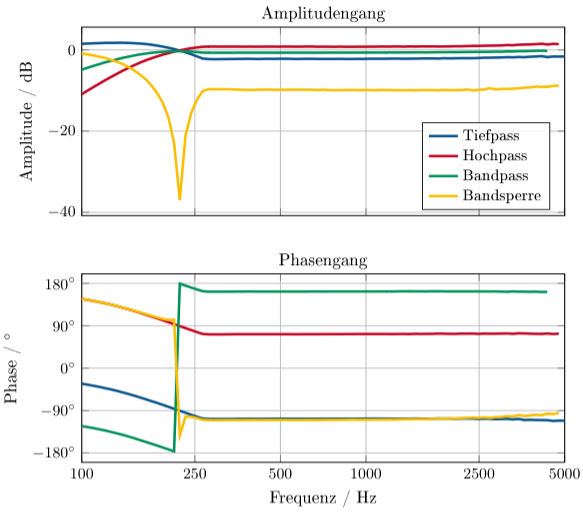
\includegraphics[width=0.8\linewidth]{../Bilder/mess_ges_sys_ac.png}
    \caption{Amplituden und Phasenverläufe der Filter im Gesamtsystem}
    \label{fig:ges_sys_out_ac}
\end{figure}

%\begin{figure} [H]
%  \centering
%    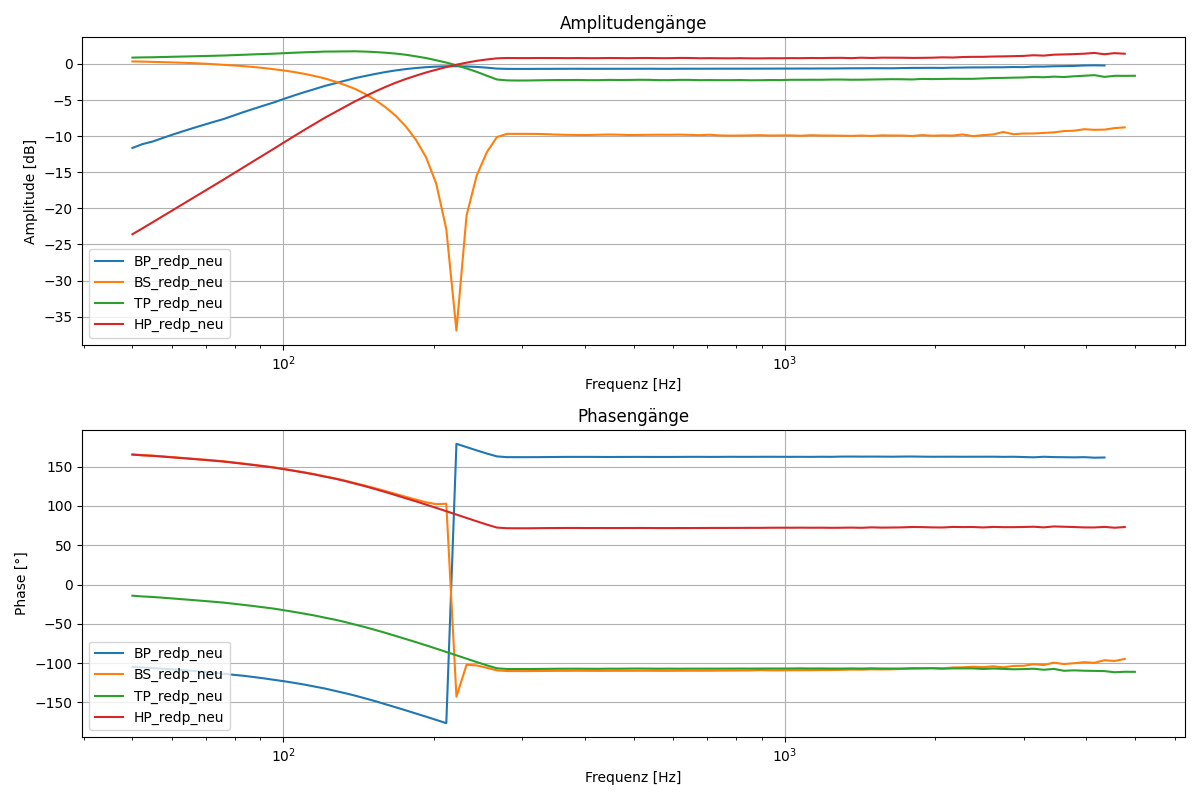
\includegraphics[width=0.8\linewidth]{../Bilder/Messung_ges_sys_ac.png}
%    \caption{Amplituden und Phasenverläufe der Filter im Gesamtsystem}
%    \label{fig:ges_sys_out_ac}
%\end{figure}

Zusätzlich weichen die Frequenzverläufe von den charakterischtischen Verläufen ab. Der Amplitudenverlauf der Bandsperre zeigt im zweiten Durchlassbereich eine Dämpfung von etwa 8 bis \SI{10}{\decibel}. Der Phasenverlauf zeigt zudem kurz vor dem Sprung an der Mittenfrequenz eine starke Erhöhung anstatt wie in der Simulation weiter zu fallen. Am Bandpass tritt im höheren Frequenzbereich keine Dämpfung mehr auf und verhält sich entsprechend eines Hochpasses. Die Flankensteilheit am Tiefpass ist deutlich zu gering, sodass dieser eher einem Allpass entspricht.\par
\medskip

Zusammenfassend lässt sich feststellen, dass dem System die notwendige Dämpfung im höheren Frequenzbereich fehlt, wobei lediglich der Hochpass (HP) einen korrekten Verlauf beibehält.\par
\medskip

\textbf{Hypothese: diese Messmethode kann nicht mit einem solchen system gemessen werden. es sieht etwas so aus, als ob der Filter versucht hinter der eingehenden frequenz herzukommen nach erreichen der Resonanzfrequenz}\par
\medskip

Um die Ursache für die Inkonsistenzen einzugrenzen, soll der \gls{vcf} ohne Einfluss durch den Phasendetektor betrachtet werden. Durch das Entfernen von $R_{10}$ wird der Regelkreis von der Phasendetektion getrennt. Die Steuerspannung $V_c$ wird auf ein definiertes Potential von \SI{1}{\volt} gesetzt. \par
\medskip


\begin{figure} [H]
  \centering
    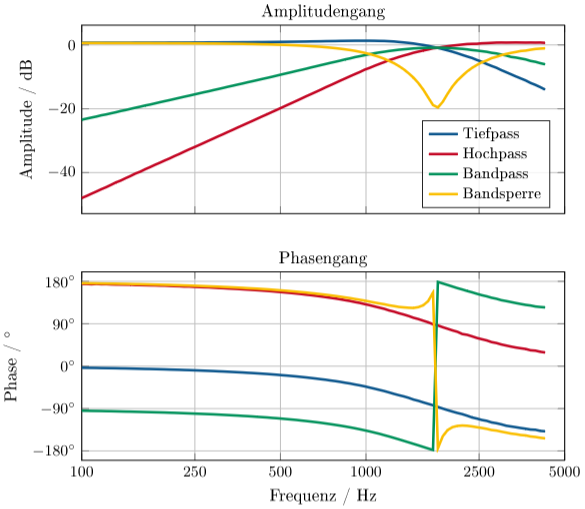
\includegraphics[width=0.8\linewidth]{../Bilder/mess_vcf_ac.png}
    \caption{Amplituden und Phasenverläufe der Filter des VCF}
    \label{fig:vcf_out_ac}
\end{figure}



%\begin{figure} [H]
%  \centering
%    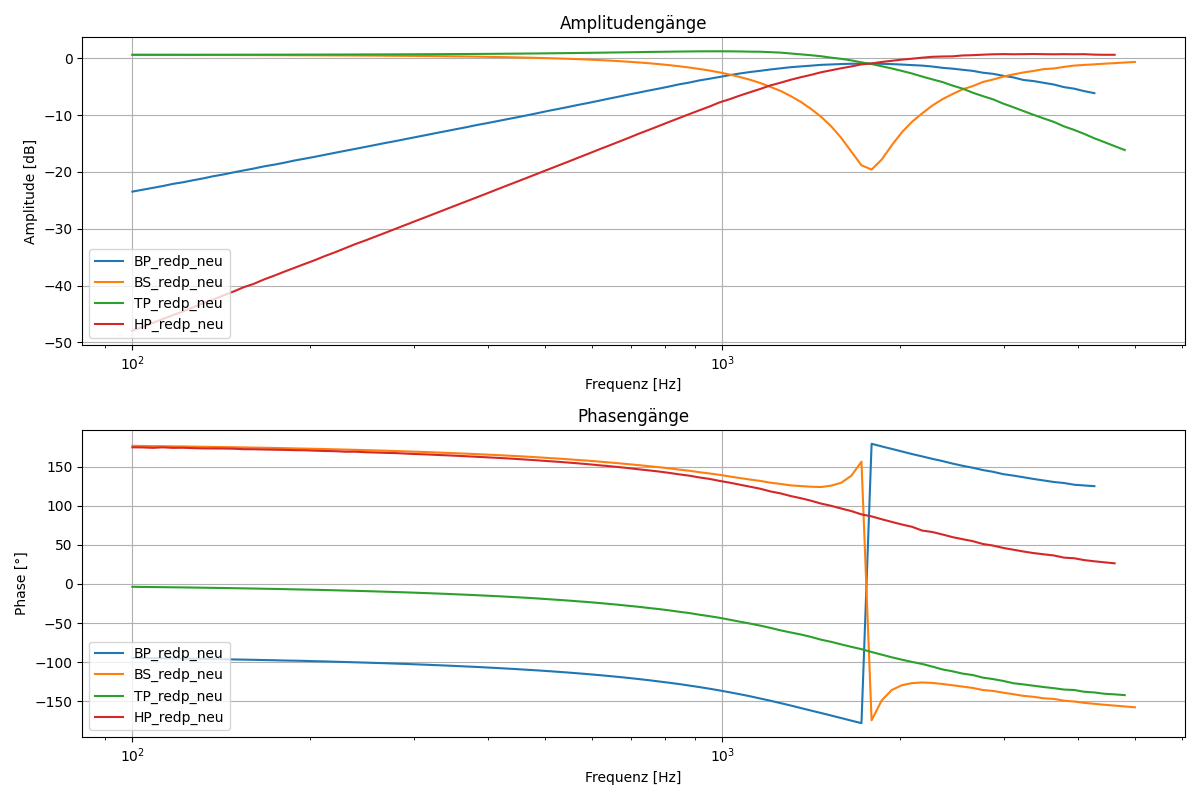
\includegraphics[width=0.8\linewidth]{../Bilder/Messung_vcf_ac.png}
%    \caption{Amplituden und Phasenverläufe der Filter des VCF}
%    \label{fig:vcf_out_ac}
%\end{figure}


Auf den ersten Blick scheinen die Verläufe der Ausgänge korrekt zu sein, sodass mit der tieferen Analyse der Mittenfrequenz begonnen werden kann.\par
\medskip


\subsection*{Experimentelle Verifizierung der Mittenfrequenzgleichung}
\label{sec:veri_omega0}
Für den herkömmlichen Biquad ligt die Mittenfrequenz für $R= \SI{1}{\kilo\ohm}$ und $C= \SI{1}{\micro\farad}$ bei etwa \SI{160}{\hertz}. Bei gleichen Parametern liegt $f_0$ für den \gls{vcf} deutlich höher. Das liegt daran, dass mit der Veränderung des Schaltungsaufbaus auch die Zusammensetzung der Mittenfrequenz beeinflusst wird. Die Mittenfrequenz des herkömmlchen Biquads ist als $\omega_0 = \frac{1}{RC}$ (Gleichung \ref{eq:w_0}) definiert, während für den \gls{vcf}-Aufbau die Referenzspannung $V_r$ und Steuerspannung $V_c$ berücksichtigt werden müssen. \par
\medskip

Die in Kapitel \ref{sec:theorie_w0} hergeleiteten Mittenfrequenzen werden hier im Folgenden nocheinmal betrachtet, um zu verifizieren welche korrekt ist. Die Gleichung \par
\medskip

\begin{equation}
    \omega_0 = \frac{V_r}{V_cRC}
    \tag{\ref{eq:filtergrenzfrequenz}}
\end{equation}

wurde dabei eigenständig hergeleitet, während die Gleichung 

\begin{equation}
    \omega_0 = \frac{V_c}{V_r \cdot RC} 
    \tag{\ref{eq:freq-vcf}}
\end{equation}

aus dem ASLK-PRO Manual stammt. Wie schon zuvor erwähnt unterscheiden sich diese beiden Gleichungen nur in dem hinzugefügten Faktor aus Referenzspannung $V_r$ und Steuerspannung $V_c$. Bei Messung dieser Signale fällt auf, dass das Potential für $V_r$ bei einer Versorgungsspannung von \SI{\pm15}{\volt} auf \SI{-13.73}{\volt} liegt und nicht wie im Datenblatt angegeben auf \SI{-10}{\volt} lasergetrimmt ist. Bei Änderung der negativen Versorgungsspannung ist zudem zu erkennen, dass $V_r$ immer etwa \SI{1.27}{\volt} unter dieser liegt. Aus diesem Grund wird die Versorgungsspannung von \SI{\pm15}{\volt} zeitweise auf \SI{\pm11}{\volt} reduziert, um mit \SI{-9.73}{\volt} deutlich näher an den angegebenen \SI{-10}{\volt} zu liegen. In der zweiten Iteration des \gls{pcb} soll der SF Pin über einen Trimmer angepasst werden können, die erste Iteration bietet diese Funktion noch nicht.\par
\medskip  

%Bei Annahme von $V_c=\SI{1}{\volt}$ und $V_r=\SI{9.73}{\volt}$ können nun die Modelle auf Richtigkeit getestet werden. 


Für die Vermessung des \gls{vcf} werden die Filterparameter wie gewohnt gewählt. Die Widerstände liegen bei etwa \SI{1}{\kilo\ohm}, die Steuerspannung $V_c$ wird auf \SI{1}{\volt} und die Referenzspannung $V_r$ auf \SI{9.73}{\volt} eingestellt. Die visuelle Auswertung der Filterverläufe zeigt zunächst einen korrekten Verlauf, weshalb die frequenzbestimmenden Widerstände im nächsten Schritt über den gesamten Filterbereich variiert werden. Die Mittenfrequenz wird dabei über den Nulldurchgang der Phase im Bandsperrenausgang ermittelt. Die Ergebnisse sind in Tabelle \ref{tab:mittenfrequenzen} zusammengefasst.\par
\medskip

\begin{table}[h]
    \centering
    \begin{tabular}{c|c|c|c}
        \textbf{Soll-R / \si{\ohm}} & \textbf{Messung: $\omega_0$ / \si{\hertz}} & \textbf{Theorie: $\omega_0$ / \si{\hertz}} & \textbf{Abweichung / \%} \\ \hline
        1591 & 1116.22 & 973.34 & 12.8 \\
        994 & 1776.34 & 1557.93 & 12.3 \\
        796 & 2140.18 & 1945.45 & 9.1 \\
        531 & 3253.12 & 2916.34 & 10.35 \\
        318 & 5789.74 & 4869.74 & 15.89 \\
        212 & 7653.34 & 7304.61 & 4.56 \\
        159 & 11570.81 & 9739.48 & 15.83 \\
    \end{tabular}
    \caption{Mittenfrequenzen und Abweichungen mit Elektrolytkondensatoren}
    \label{tab:mittenfrequenzen}
\end{table}

Die theoretischen Werte basieren auf der eigenständig hergeleiteten Gleichung \ref{eq:filtergrenzfrequenz}. Es zeigt sich, dass das System zwar grob der theoretischen Gleichung folgt. Die Abweichungen sind mit bis zu \SI{15.89}{\percent} jedoch noch sehr hoch. Um diese Abweichungen zu kompensieren, wird die Berechnungsfunktion für die theoretische Mittenfrequenz in Python an die gemessenen Werte angepasst. Durch die Multiplikation der Widerstandswerte mit einem Faktor von \num{0.9} lässt sich die Abweichung für die gemessenen Werte auf \SI{\pm7.5}{\percent} reduzieren, statt der ursprünglichen \SI{\pm15.89}{\percent}.\par
\medskip

Um die Ursache für diese starken Abweichungen zu verstehen, wird die Schaltung nochmals detailliert betrachtet. Dabei fällt auf, dass die verbauten Elektrolytkondensatoren eine Toleranz von bis zu \SI{20}{\percent} aufweisen. Obwohl die Bauteiltoleranzen in einem Self-Tuned Filter theoretisch nur eine untergeordnete  Rolle spielen sollten, ist es für präzise Messungen an Teilsystemen wie dem \gls{vcf} vorteilhaft, geringere Toleranzen zu haben. Aus diesem Grund werden die Elektrolytkondensatoren gegen Folienkondensatoren ausgetauscht, die eine Toleranz von nur \SI{5}{\percent} aufweisen.\par
\medskip

\begin{table}[h]
    \centering
    \begin{tabular}{c|c|c|c}
        \textbf{Soll-R / \si{\ohm}} & \textbf{Messung: $\omega_0$ / \si{\hertz}} & \textbf{Theorie: $\omega_0$ / \si{\hertz}} & \textbf{Abweichung / \%} \\ \hline
        1591 & 1038.04 & 973.34 & 6.23 \\
        994 & 1656.58 & 1557.93 & 5.95 \\
        796 & 1993.77 & 1945.45 & 2.42 \\
        531 & 2960.54 & 2916.34 & 1.49 \\
        318 & 5327.21 & 4869.74 & 8.59 \\
        212 & 6863.27 & 7304.61 & -6.43 \\
        159 & 9930.13 & 9739.48 & 1.92 \\
    \end{tabular}
    \caption{Mittenfrequenzen und Abweichungen mit Folienkondensatoren}
    \label{tab:mittenfrequenzen2}
\end{table}

Wie in Tabelle \ref{tab:mittenfrequenzen2} dargestellt verbessert sich die Abweichung zwischen den Theorie- und Praxiswerten nach Austausch der Kondensatoren deutlich. Für die betrachteten Datenpunkte reduziert sich die maximale Abweichung auf unter \SI{8.6}{\percent}, was fast einer Halbierung der vorherigen maximalen Abweichung entspricht. Die verbleibende Abweichung lässt sich nicht einfach durch Skalierung eines Filterparameters verringern, da die größte negative Abweichung bei \SI{-6.43}{\percent} liegt. So wird diese auf die Bauteiltoleranzen, besonders die Digitalpotentiometer zurückzuführen sein. \par
\medskip


\textbf{vielleich ist es besser diesen teil vor den anderen zu packen. in dem davor wird ja schon von der selbst hergeleiteten gleicung ausgegangen}

Zuletzt sollen nun noch die gegensätzlichen Mittenfrequenzgleichung überprüft werden. Für die Steuerspannung wird dabei ein Wert von $V_c = \SI{1}{\volt}$ eingesetzt, die Referenzspannung beträgt $V_r = \SI{9.73}{\volt}$. Werden diese Werte nun in die beiden Gleichungen eingesetzt ergibt sich folgendes Bild:\par
\medskip

\begin{equation}
    f_0 = \frac{V_r}{V_c \cdot 2\pi RC} = \frac{\SI{9.73}{\volt}}{\SI{1}{\volt} \cdot 2\pi \cdot \SI{994}{\ohm} \cdot \SI{1}{\micro\farad}} = \SI{1557.93}{\hertz}
\end{equation}

\begin{equation}
    f_{0\_ASLK} =  \frac{V_c}{V_r \cdot 2\pi RC} = \frac{\SI{1}{\volt}}{\SI{9.73}{\volt} \cdot 2\pi \cdot \SI{994}{\ohm} \cdot \SI{1}{\micro\farad}} = \SI{16.46}{\hertz}
\end{equation}

Während die Gleichung aus dem ASLK-PRO Manual eine Mittenfrequenz von nur \SI{16.46}{\hertz} vorhersagt, liefert die eigenständig hergeleitete Gleichung einen Wert von \SI{1557.93}{\hertz}, der besser mit dem gemessenen Wert von \SI{1657}{\hertz} übereinstimmt.\par
\medskip

Um die Abhängigkeit der Mittenfrequenz von der Steuerspannung endgültig zu bestätigen, wird $V_c$ im Experiment von \SI{1}{\volt} auf \SI{2}{\volt} erhöht. Nach der Rechenvorschrift \ref{eq:filtergrenzfrequenz} sollte sich die Mittenfrequenz dadurch halbieren. Die Ergebnisse sind in Tabelle \ref{tab:mittenfrequenzen3} zusammengefasst:\par
\medskip


\begin{table}[h]
    \centering
    \begin{tabular}{c|c|c|c}
        \textbf{$V_c$ / \si{\volt}} & \textbf{Theorie: $\omega_0$ / \si{\hertz}} & \textbf{Messung: $\omega_0$ / \si{\hertz}} & \textbf{Abweichung / \%} \\ \hline
        1 & 1557.93 & 1656.58 & 5.95 \\
        2 & 778.96 & 824.39 & 5.51\\
    \end{tabular}
    \caption{Vergleich der Mittenfrequenz bei Variation von $V_c$}
    \label{tab:mittenfrequenzen3}
\end{table}

Dadurch kann bestätigt werden, dass die eigenständig hergeleitete Gleichung \ref{eq:filtergrenzfrequenz} die Mittenfrequenz für diesen \gls{vcf} korrekt beschreibt. Die Abweichungen zwischen Theorie und Messung liegen im akzeptablen Bereich und sind vermutlich auf die Toleranzen der verwendeten Bauteile zurückzuführen.\par
\medskip

(\textbf{Überleitung zu den ergebnissen aus der Sim}
Auch die Simulation des Filters in LTspice kommt auf eine andere Mittenfrequenz. diese liegt bei etwa \SI{1.76}{\kilo\hertz}. dabei sind alle schaltungsteile gleich, nur die Versorgungs und Hilfsspannungen müssen nochmals überprüft werden. \textbf{überarbeiten})\par
\medskip





\subsection*{Charakterisierung des Phasendetektors}
Nach der Vermessung des spannungsgesteuerten Filters folgt nun die Einzelbetrachtung des Phasendetektors. Dabei werden wie schon in Kapitel \ref{sec:theorie_pd} zwei Signale auf die Eingänge des \gls{pd} gegeben. Das Referenzsignal mit \SI{1000}{\hertz} und ein Messsignal mit \SI{1100}{\hertz}. Am Ausgang des Multiplizierers ergibt sich das in Abbildung \ref{fig:mult_out_osc} dargestellte Signal.\par
\medskip


\begin{figure} [H]
  \centering
    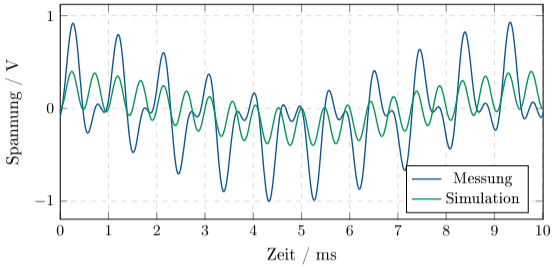
\includegraphics[width=0.8\linewidth]{../Bilder/mult_out_osc.png}
    \caption{Ausgangssignal des Mulitplizierers im Phasendetektor}
    \label{fig:mult_out_osc}
\end{figure}


%\begin{figure} [H]
%  \centering
%    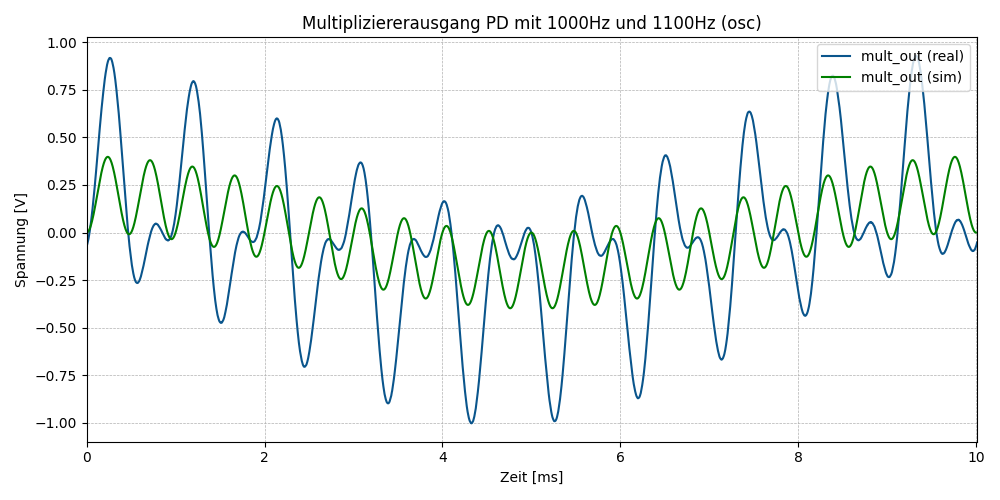
\includegraphics[width=0.8\linewidth]{../Bilder/mult_out_osc2.png}
%    \caption{Ausgangssignal des Mulitplizierers im Phasendetektor}
%    \label{fig:mult_out_osc}
%\end{figure}

Zu Beginn haben die Eingangssignale eine Phasendrehung von \SI{0}{\degree} zu einander. Wie schon in der Simulation betrachtet weist das Ausgangssignal dabei einen positiven Offset auf, der jedoch mit zunehmender Phasendifferenz stetig kleiner wird. Bei einer Verschiebung von etwa \SI{90}{\degree} geht der Offset in den negativen Bereich über. \par
\medskip

Die hochfrequente Welligkeit (Ripple) des realen Signals ist hingegen ungleichmäßiger als im idealisierten Modell. Dies lässt sich auf Nichtlinearitäten des analogen Multiplizierers zurückführen, die neben der Summenfrequenz und der Differenzfrequenz (\SI{100}{\hertz}) zusätzliche Oberschwingungen generieren. Da für die Funktion des Phasendetektors vor allem der niederfrequente Anteil relevant ist, werden diese höherfrequenten Störungen durch das Tiefpassverhalten des nachfolgenden Integrators gedämpft. Des Weiteren ist die Amplitude des Messsignals deutlich höher als in der Simulation, was auf die unterschiedlichen Eingangsamplituden (\SI{5}{\volt_{pp}} in der Messung gegenüber \SI{4}{\volt_{pp}} in der Simulation) zurückzuführen ist. \par 
\medskip

Im Allgemeinen zeigt der zeitliche Verlauf der Steuerspanung $V_c$ eine hohe Übereinstimmung zwischen Messung und Simulation.\par
\medskip


\begin{figure} [H]
  \centering
    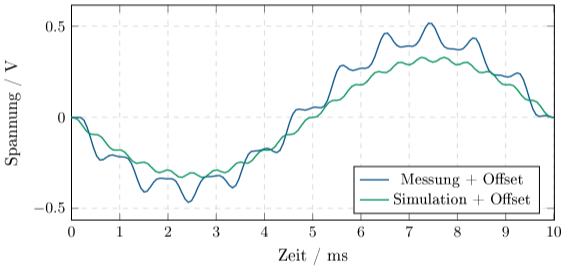
\includegraphics[width=0.8\linewidth]{../Bilder/pd_out_osc.png}
    \caption{Ausgangssignal des Phasendetektors (AC-Betrachtung)}
    \label{fig:pd_out_osc}
\end{figure}

%\begin{figure} [H]
%  \centering
%    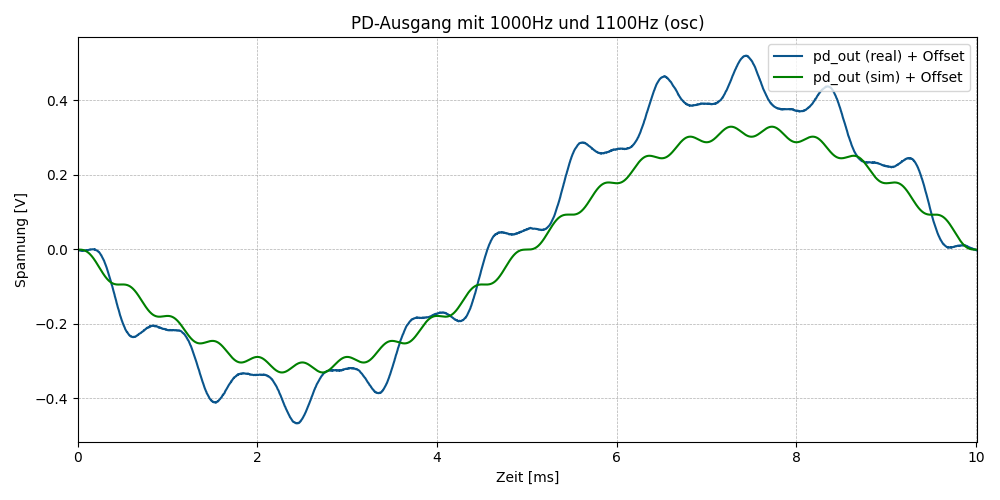
\includegraphics[width=0.8\linewidth]{../Bilder/pd_out_osc2.png}
%    \caption{Ausgangssignal des Phasendetektors (AC-Betrachtung)}
%    \label{fig:pd_out_osc}
%\end{figure}

Der allgemeine Vergleich der Signalverläufe nach dem Integrator zeigt eine hohe Übereinstimmung zwischen Simulation und Messung. Die restliche Welligkeit ist auf die zuvor beschriebene unsaubere Multiplikation zurückzuführen. Der signifikanteste Unterschied zwischen den beiden Signalen liegt im DC-Offset. Das Simulationssignal besitzt einen Gleichanteil von \SI{2.528}{\volt}, während die Messung mit \SI{13.68}{\volt} DC belegt ist. \textbf{Dieser Versatz ist mit  xxx zu erklären. warum?}. Zudem ist eine geringe Phasenverschiebung zwischen den Funktionen erkennbar.\par
\medskip

Trotz dieser Abweichungen ist die grundlegende Funktionalität des Phasendetektors gegeben, da die Signalform dem Idealverlauf entspricht. Somit ist belegt, dass beide Teilschaltungen, der spannungsgesteuerte Filter sowie der Phasendetektor, einzeln betrachtet funktionstüchtig sind. Im Folgenden kann daher das Gesamtsystem untersucht werden. \par
\medskip






\subsection{Sprungantwort des Self-Tuned Filters}
Die in der Simulation analysierte Frequenz-Sprungantwort soll nun durch eine experimentelle Messung am realen System widerholt werden. Dabei soll das Signal am Eingang des \gls{dut} schnell zwischen zwei Frequenzen wechseln, um die Reaktion des Systems auf diesen plötzlichen Frequenzwechsel zu beobachten. \par
\medskip

Dazu wird das \gls{dut} mit einem Signalgenerator angesteuert, der über die \gls{fsk}-Modulation einen automatischen Frequenzwechsel ausgibt. Bei dieser Modulationsart werden eine Grundfrequenz und eine Carrierfrequenz festgelegt, zwischen denen Ausgangssignal des Generators in einem vorgegebenen Takt umschaltet.\par
\medskip

Da der genaue Stabilitätsbereich für die Frequenzsprünge am realen System unbekannt ist, gibt der Signalgenerator anfangs die Frequenzen \SI{750}{\hertz} und \SI{3}{\kilo\hertz} aus. Die nach der Einschwingphase gemessenen Potentiale der Steuerspannung $V_c$ und die daraus resultiertende Resonanzfrequenz $f_0$ liegen bei \SI{620}{\hertz} und \SI{2770}{\hertz}. Trotz dieser Abweichung folgt das System der eingehenden Frequenz. Eine detaillierte Analyse dieser Ergebnisse erfolgt in Kapitel \ref{sec:ausw_sprung}.\par
\medskip

Bei der Messung der Sprungantwort fällt zudem auf, dass je nach Taktrate des Frequenzwechsels Atefakte entstehen. Dabei übersteuert die Amplitude des Filterausgangssignals stark, sodass statt einer Spitzenspannung von $V_p= \SI{1}{\volt}$ Werte von \SI{9.5}{\volt} erreicht werden. Dieses Verhalten tritt immer beim Sprung von der niedrigen auf die hohe Frequenz auf, wobei die Amplitude entweder nach kurzer Zeit wieder auf den Normalwert fällt oder sich über mehrere Perioden streckt. Das Fallen auf den Normalwert erfolgt dabei ebenso aprupt wie das Auftreten der Überhöhung. Bei geringer Taktfrequenz (\SI{1}{\hertz}) treten diese Überhöhungen kaum auf. Wird der Takt jedoch auf beispielsweise \SI{10}{\hertz} erhöht, können auch die Amplitudenübersteuerungen häufiger beobachtet werden.\par
\medskip

\begin{figure} [H]
  \centering
    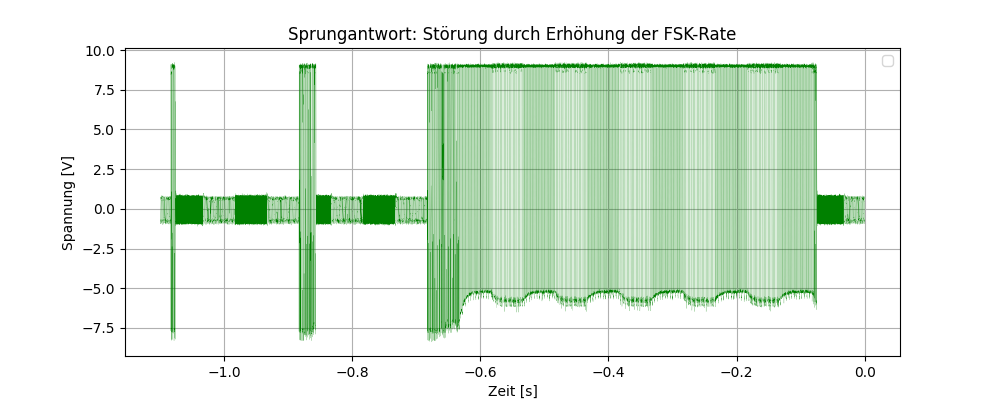
\includegraphics[width=1\linewidth]{../Bilder/sprung_stör_FSK.png}
    \caption{Bild der Störung}
    \label{fig:sprung_mess_FSK}
\end{figure}


Um die Ursache für die Amplitudenübersteuerungen besser einzugrenzen, wird die Platine mittels Druckluft heruntergekühlt. Damit soll eine Temperaturabhängigkeit, wie beispielsweise die Überhitzung einzelner Bauteile, ausgeschlossen werden. Das Abkühlen zeigte anfangs einen positiven Effekt auf die Häufigkeit der Artefakte, jedoch konnte dies bei wiederholter Kühlung nicht reproduziert werden. \par
\medskip

Um zudem die \glspl{opv} als Fehlerquelle ausschließen zu können, wurden die ursprünglichen TL082B gegen pinkompatible LM358 ausgetauscht. Diese besitzen eine geringere Slew-Rate sowie ein kleineres \gls{gbw}, reagieren also langsamer als der TL082. In der Messung stieg die Fehlerrate durch den Austausch der \glspl{opv} noch weiter an. \textbf{Es fehlt noch ein kurzer Grund für die Maßnahme. Evtl. in Richtung um das Verhalten anderer Vergleichbarer OPVs zu testen. Ob das BAuteil oder das System die Schwingungen erzeugt.  }\par
\medskip

Für einen weiteren Test mit einem AD8062 wurde die Versorgungsspannung der Platine auf \SI{\pm8}{\volt} gesenkt, um die Grenzwerte des Bauteils einzuhalten. Leider liefert auch diese Messung keine konsitstenten Ergebnisse. Dabei zeigte sich, dass der \gls{opv} das Ausgangssignal stark zum schwingen bringt. Eine mögliche Ursache dafür ist, dass die Schaltung nicht für einen so schnellen \gls{opv} ausgelegt ist.\par
\medskip 


Die auf die tatsächliche Ursache wird ausführlich in der Auswertung eingegangen.\par
\medskip





\subsection{Einschwingbereich des Filters}

Trotz der geringen Aussagekraft der Simultationsergebnisse soll zur Vervollständigung auch das reale System über einen Frequenzsweep vermessen werden. Dafür wird der Signalgenerator im entsprechenden Betriebsmodus verwendet, wobei nur die Start- und Stoppfrquenz sowie die Dauer des Sweeps angegeben werden müssen. Das Ergebnis kann dann über das Oszilloskop mit einer entsprechned eingestellten Sample Time aufgenommen werden.\par
\medskip

Zusätzlich wird der Einschwingbereich über den Aufbau für die Sprungantwort vermessen. Durch die schrittweise Erhöhung beziehungsweise Verringerung der Eingangsfrequenz kann so die Frequenz ermittelt werden bei der sich das System nicht mehr selbständig einfangen kann. \par
\medskip




%Aufnahme über spektrum analysator? Herausfinden wie groß der Filter/ Einstellungsbereich des Filters ist. Also bis zu welcher abweichung von eingehender Freq und bauteilbedingter Mittenfreq. der filter noch die win=w0 schafft. 

\end{document}
